
The event yields from different event categories with systematics and 
statistical uncertainties are shown in Table~\ref{tab:eventYieldInc},
\ref{tab:eventYieldCTagInc}, and \ref{tab:eventYieldCTagEx} for 
\mujets and \ejets channel. From these tables, it can 
be seen that the total background event matches well with the data 
within the uncertainties. In view of this, an expected exclusion limit 
with 95\% CL has been put on the \brThb, assuming \brHcs = 100\%.

The absence of a charged Higgs boson signal in the 
data is characterized by setting exclusion limits on the branching 
fraction \Bthb. 
An asymptotic 95\% \CL limit on \Bthb is 
calculated using the \CLs method~\cite{Junk:1999kv,Read:2002hq} with
likelihood ratios~\cite{Cowan:2010js}:
\begin{linenomath}
\begin{equation}
    \widetilde{q}_{x} = -2 \ln \frac{\mathcal{L}(\text{data}|x,
    \hat{\Uptheta}_{x})}{\mathcal{L}(\text{data}|\hat{x},\hat{\Uptheta})}.
\end{equation}  
\end{linenomath}
where the likelihood is defined as 
\begin{linenomath}
\begin{equation}
    \mathcal{L}(\text{data}|x,\Uptheta) = \prod_{j=1}^{3}\prod_{i=1}^{N}\frac{N_{ij}(x, 
    \Uptheta)^{n_{ij}}}{n_{ij}!}\re^{-N_{ij}(x, \Uptheta)} \prod_k
    p(\widetilde{\Uptheta}_k|\Uptheta_k).
\label{eq:likelihood}
\end{equation}
\end{linenomath}

In this equation, $x = \Bthb$ is the parameter of interest, the first product over
$j$ designates the three charm tagging categories, and $i$ runs over the bins of the \mjj distributions shown
in Fig.~\ref{fig:mjj_cTagEx}. For a given mass bin $i$ and charm tagging category $j$, $n_{ij}$ is the
observed number of events in that bin and charm tagging category, and $N_{ij}(\Uptheta)$ is the expected
number of events. The last term is the product over the individual nuisance parameters $k$ of the probability
density function $p(\widetilde{\Uptheta}_k|\Uptheta_k)$, where $\Uptheta_k$ is the value of the nuisance
parameter.  The estimators $\hat{x}$ and $\hat{\Uptheta}$ correspond to the global maximum of the likelihood
defined in Eq.~\ref{eq:likelihood}. The expected number of events $N_{ij}(\Uptheta)$ is given by, in the
presence of signal:
\begin{linenomath}
\ifthenelse{\boolean{cms@external}}
{\begin{multline}
\label{nbsm}
N_{ij}(x,\Uptheta) = 2x(1-x)N_{ij}^{\ttbar \to \PSHp \PWm}(\Uptheta) \\
+(1-x)^2 N_{ij}^{\ttbar\to \PW^{\pm}\PW^{\mp}}(\Uptheta) + 
N_{ij}^{\text{other}}(\Uptheta),
\end{multline}}
{\begin{equation}
\label{nbsm}
N_{ij}(x,\Uptheta) = 2x(1-x)N_{ij}^{\ttbar \to \PSHp \PWm}(\Uptheta) + 
(1-x)^2 N_{ij}^{\ttbar\to \PW^{\pm}\PW^{\mp}}(\Uptheta) + 
N_{ij}^{\text{other}}(\Uptheta),
\end{equation}}
\end{linenomath}
and in the absence:
\begin{linenomath}
   \begin{equation}
       N_{ij}(\Uptheta) = N_{ij}^{\ttbar \to \PW^{\pm}\PW^{\mp}}(\Uptheta) + N_{ij}^{\text{other}}(\Uptheta),
   \end{equation}
   \end{linenomath}
where $N_{ij}^{\ttbar\to \PSHp\PWm}(\Uptheta)$ and $N_{ij}^{\ttbar \to \PW^{\pm}\PW^{\mp}}(\Uptheta)$ are the
number of events from the simulated signal process and the SM \ttbar process, respectively. Both are
normalized to the expected \ttbar cross sections, as described in Section~\ref{s:secDataMC}. The factor of 2
in Eq.~\ref{nbsm} is derived from the assumption that the event yield and \Bthbbar for \PSHm are the same as
those of \PSHp.

%-----------------------------------------
\subsection{Limits from inclusive event category without \text{c} tagging}
\label{ss:limit_Inc}
%-----------------------------------------
To extract possible signal, the $\mjj$ distribution as shown in Figures~\ref{subfig:mjj_kfit_muKinFit},~\ref{subfig:mjj_kfit_eleKinFit},~\ref{subfig:mjj_sig_kfit_mu}, and \ref{subfig:mjj_sig_kfit_ele} are used in the binned maximum-likelihood fit. The upper limit on the \brThb as a function of $m_{H^{+}}$ is 
shown in Figures~\ref{subfig:limit_mu_Inc},~\ref{subfig:limit_ele_Inc}, and \ref{subfig:limit_lep_Inc}
for the \mujets and \ejets and \ljets channel, respectively. 
Corresponding values of the expected (observed) limits, for the 
charged Higgs mass from 80 to 160 \GeV, are in the range 
0.37--4.38\% (0.44--5.29\%), 0.43--5.04\% (0.27--3.94\%), 
and 0.30--3.45\% (0.28--2.89) respectively. The expected (observed) 
limits using $\mjj$ from inclusive event category the 8 \TeV analysis, 
for the mass of charged Higgs boson in the range 90 to 160 \GeV, was 
in range 1.4--3.6\% (1.2--6.5\%) for \ljets channel~\cite{Khachatryan:2015uua}.
\begin{figure}
    \centering  
    \subfigure[Without \PQc tagging \label{subfig:limit_mu_Inc}]
    {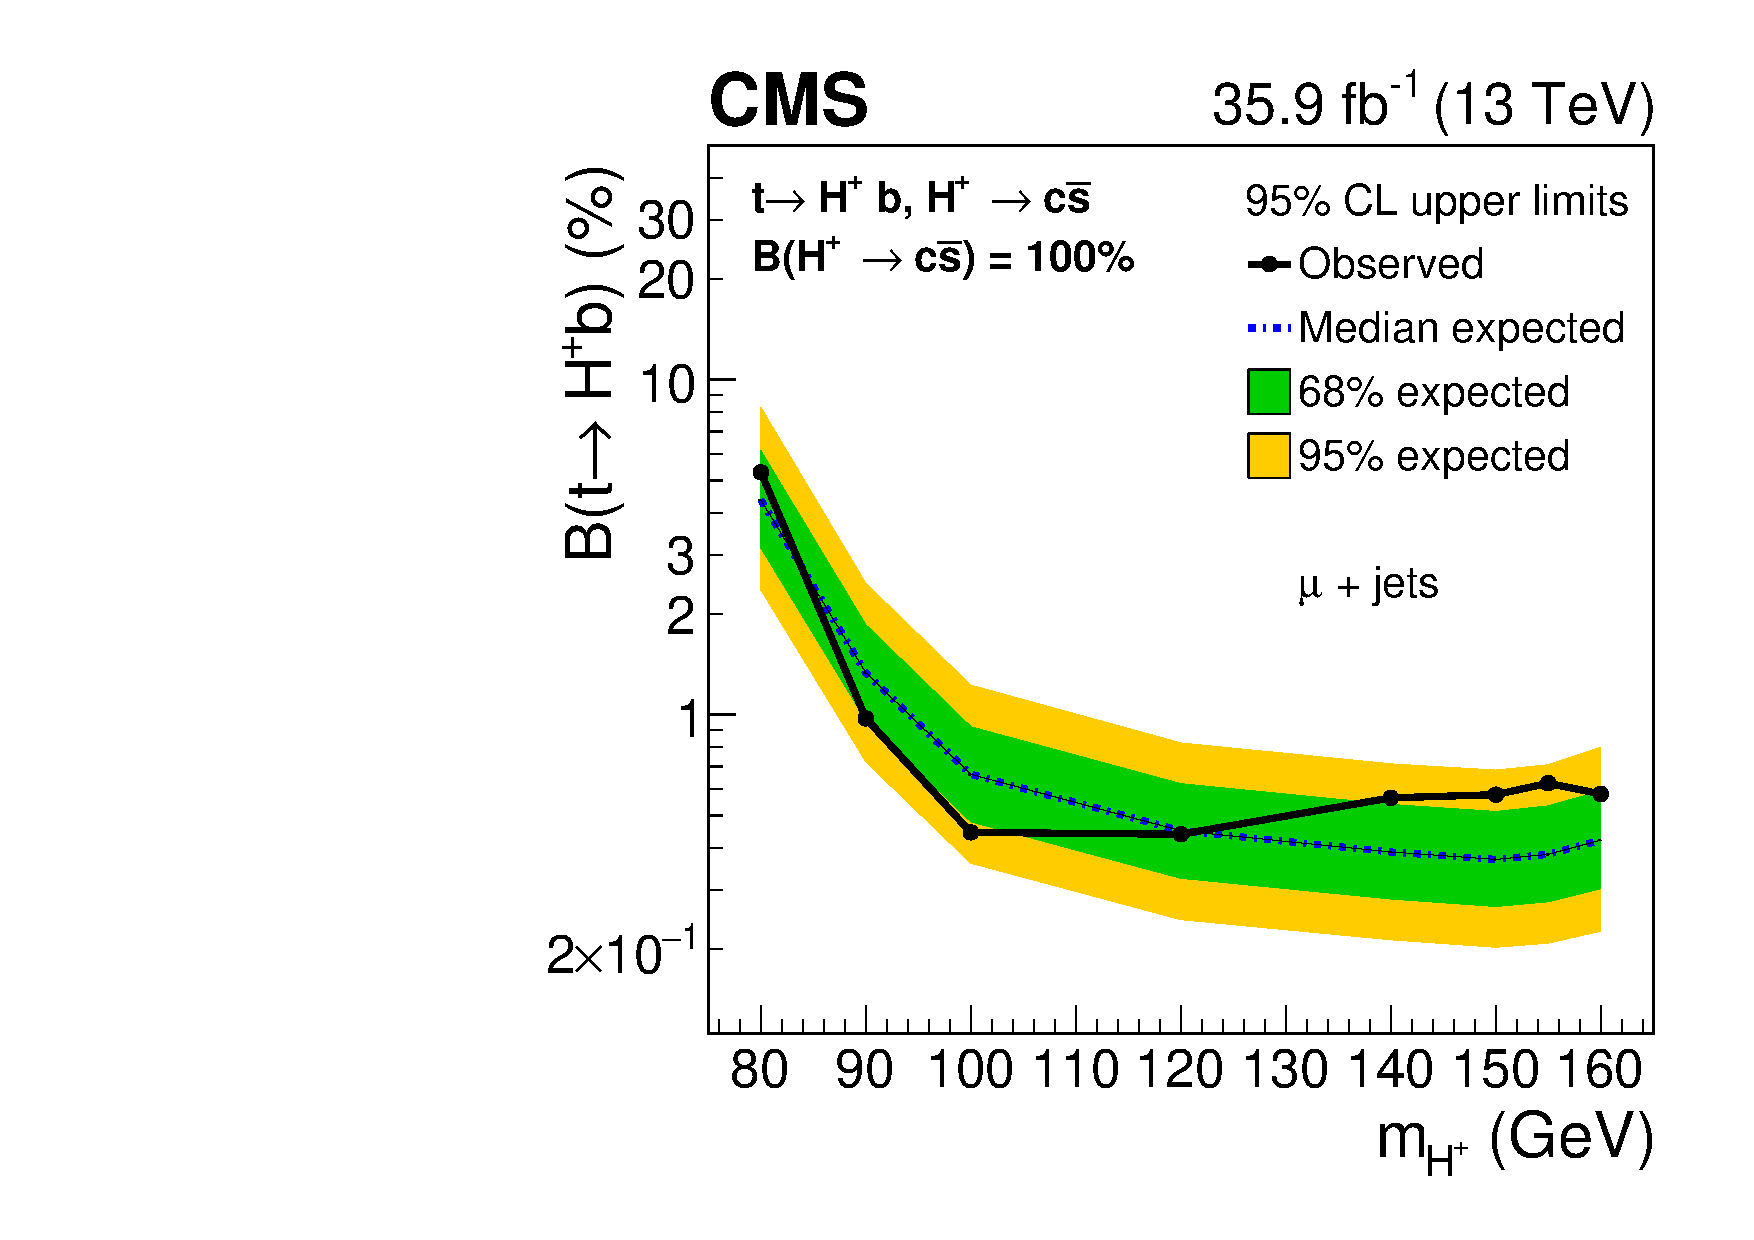
\includegraphics[width=0.30\linewidth]{Image/Limit/limit_pdf/limit_mu_Cat1_Inc.pdf}}
    \subfigure[Without \PQc tagging \label{subfig:limit_ele_Inc}]
    {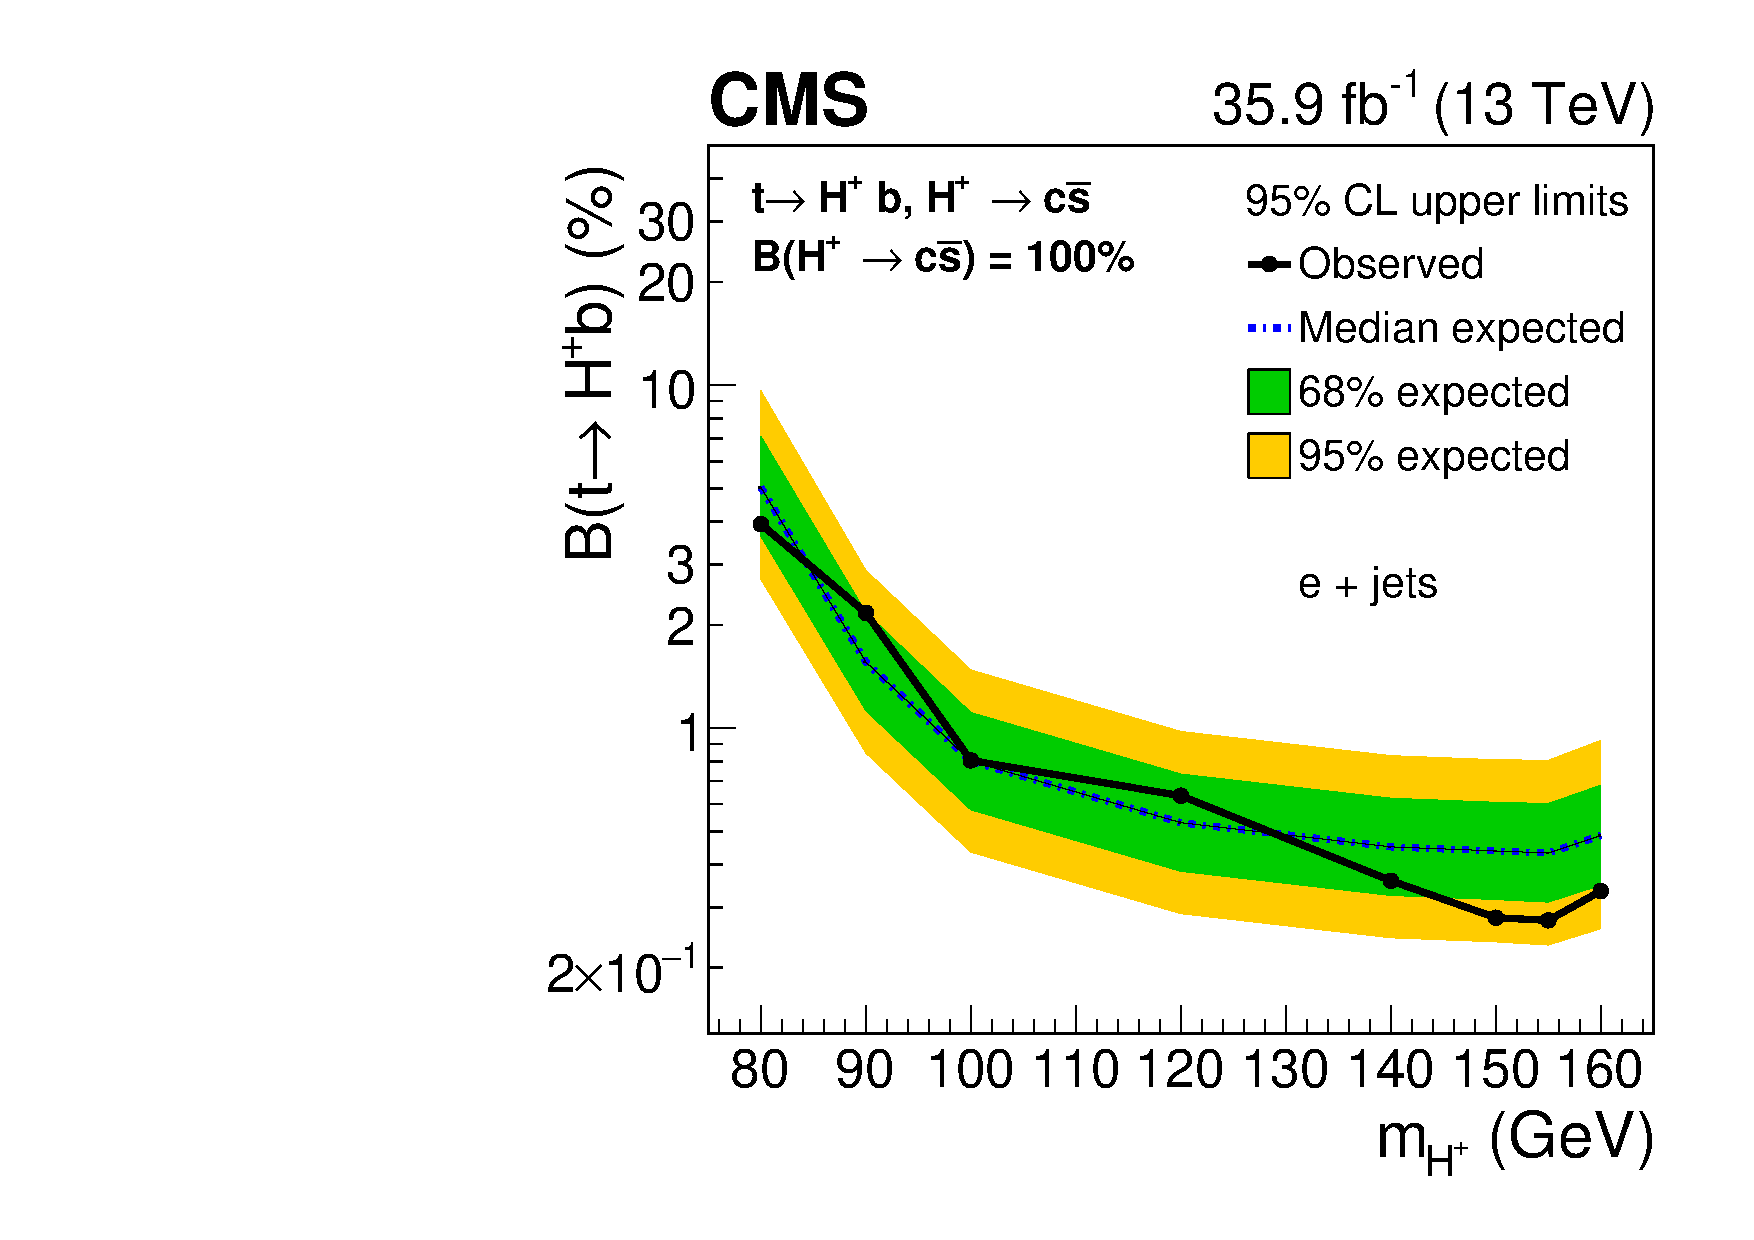
\includegraphics[width=0.30\linewidth]{Image/Limit/limit_pdf/limit_ele_Cat1_Inc.pdf}}
    \subfigure[Without \PQc tagging \label{subfig:limit_lep_Inc}]
    {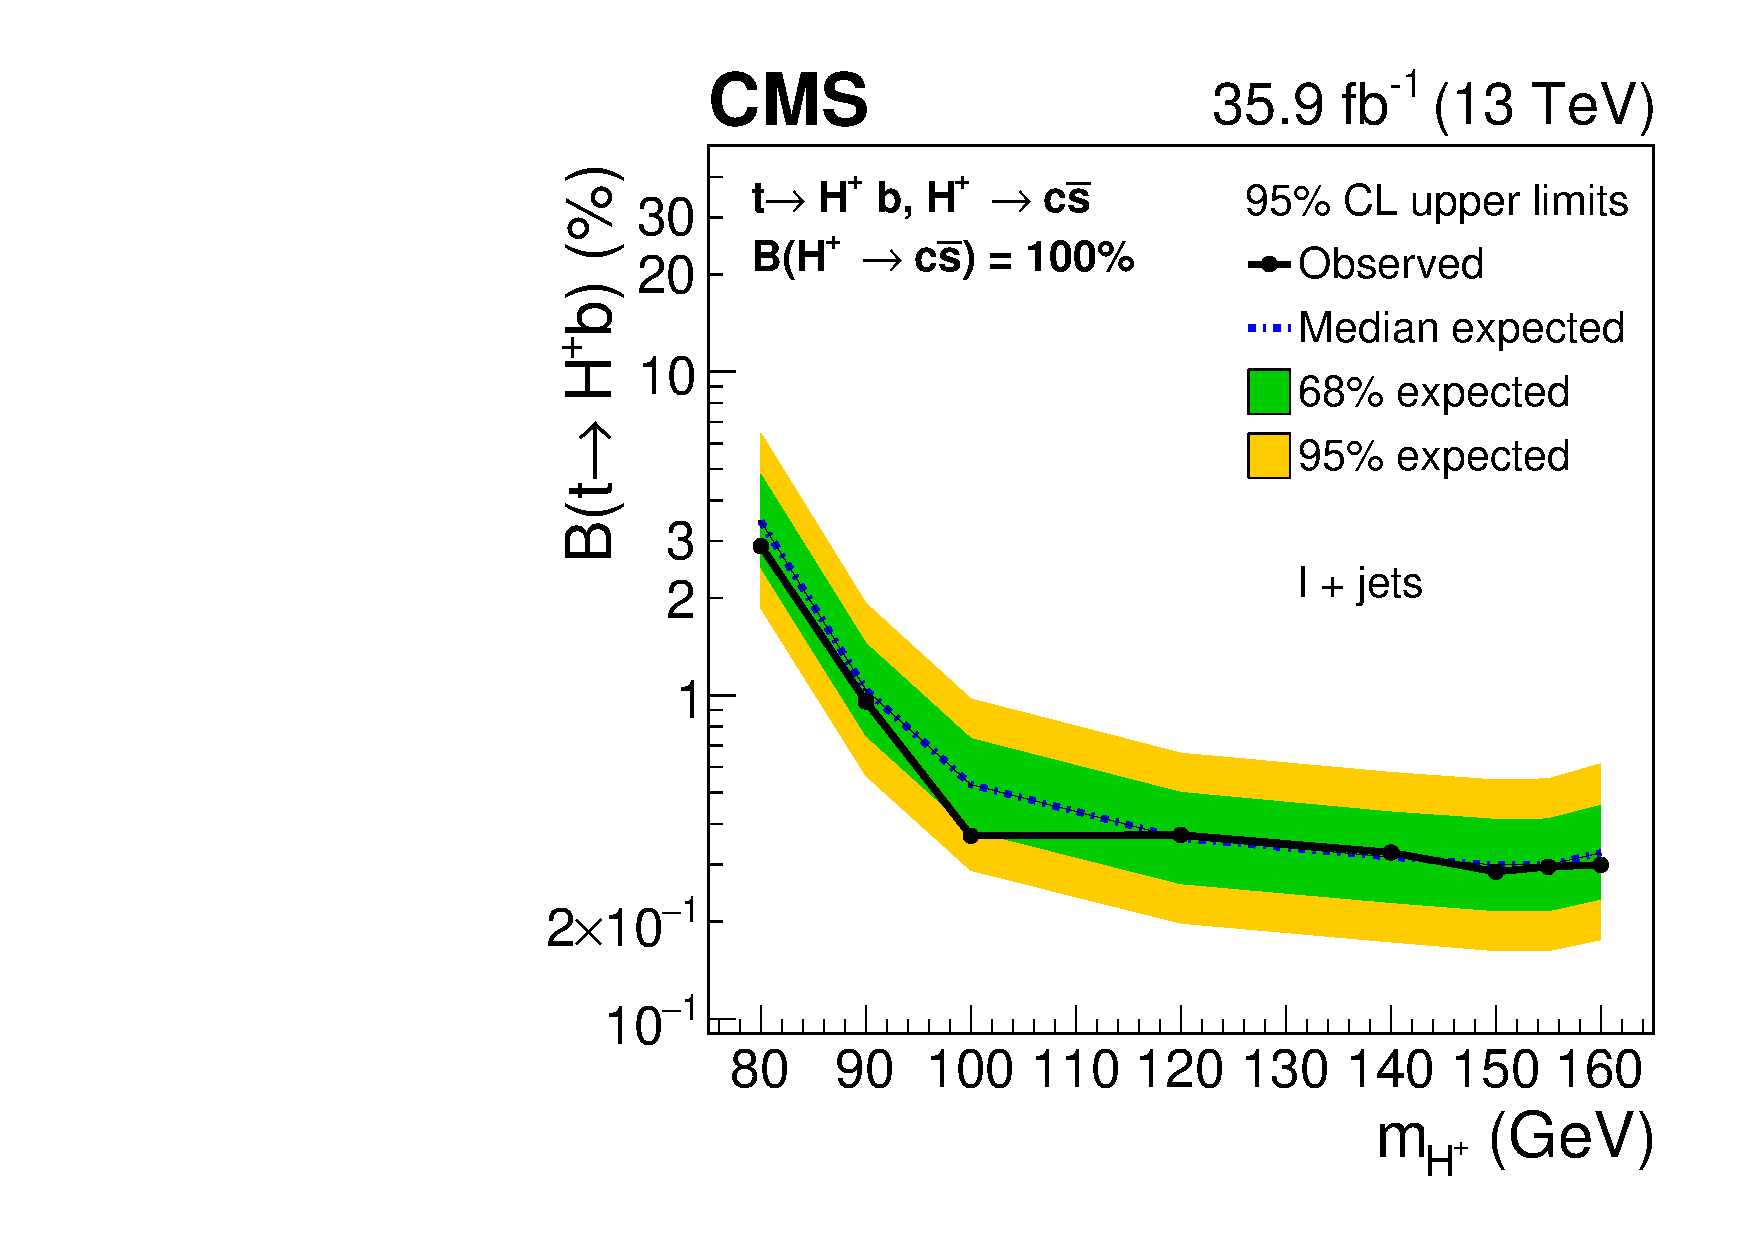
\includegraphics[width=0.30\linewidth]{Image/Limit/limit_pdf/limit_mu_ele_Cat1_Inc.pdf}}
    \vfil
    \subfigure[With loose \PQc tagging \label{subfig:limit_mu_cTagL}]
    {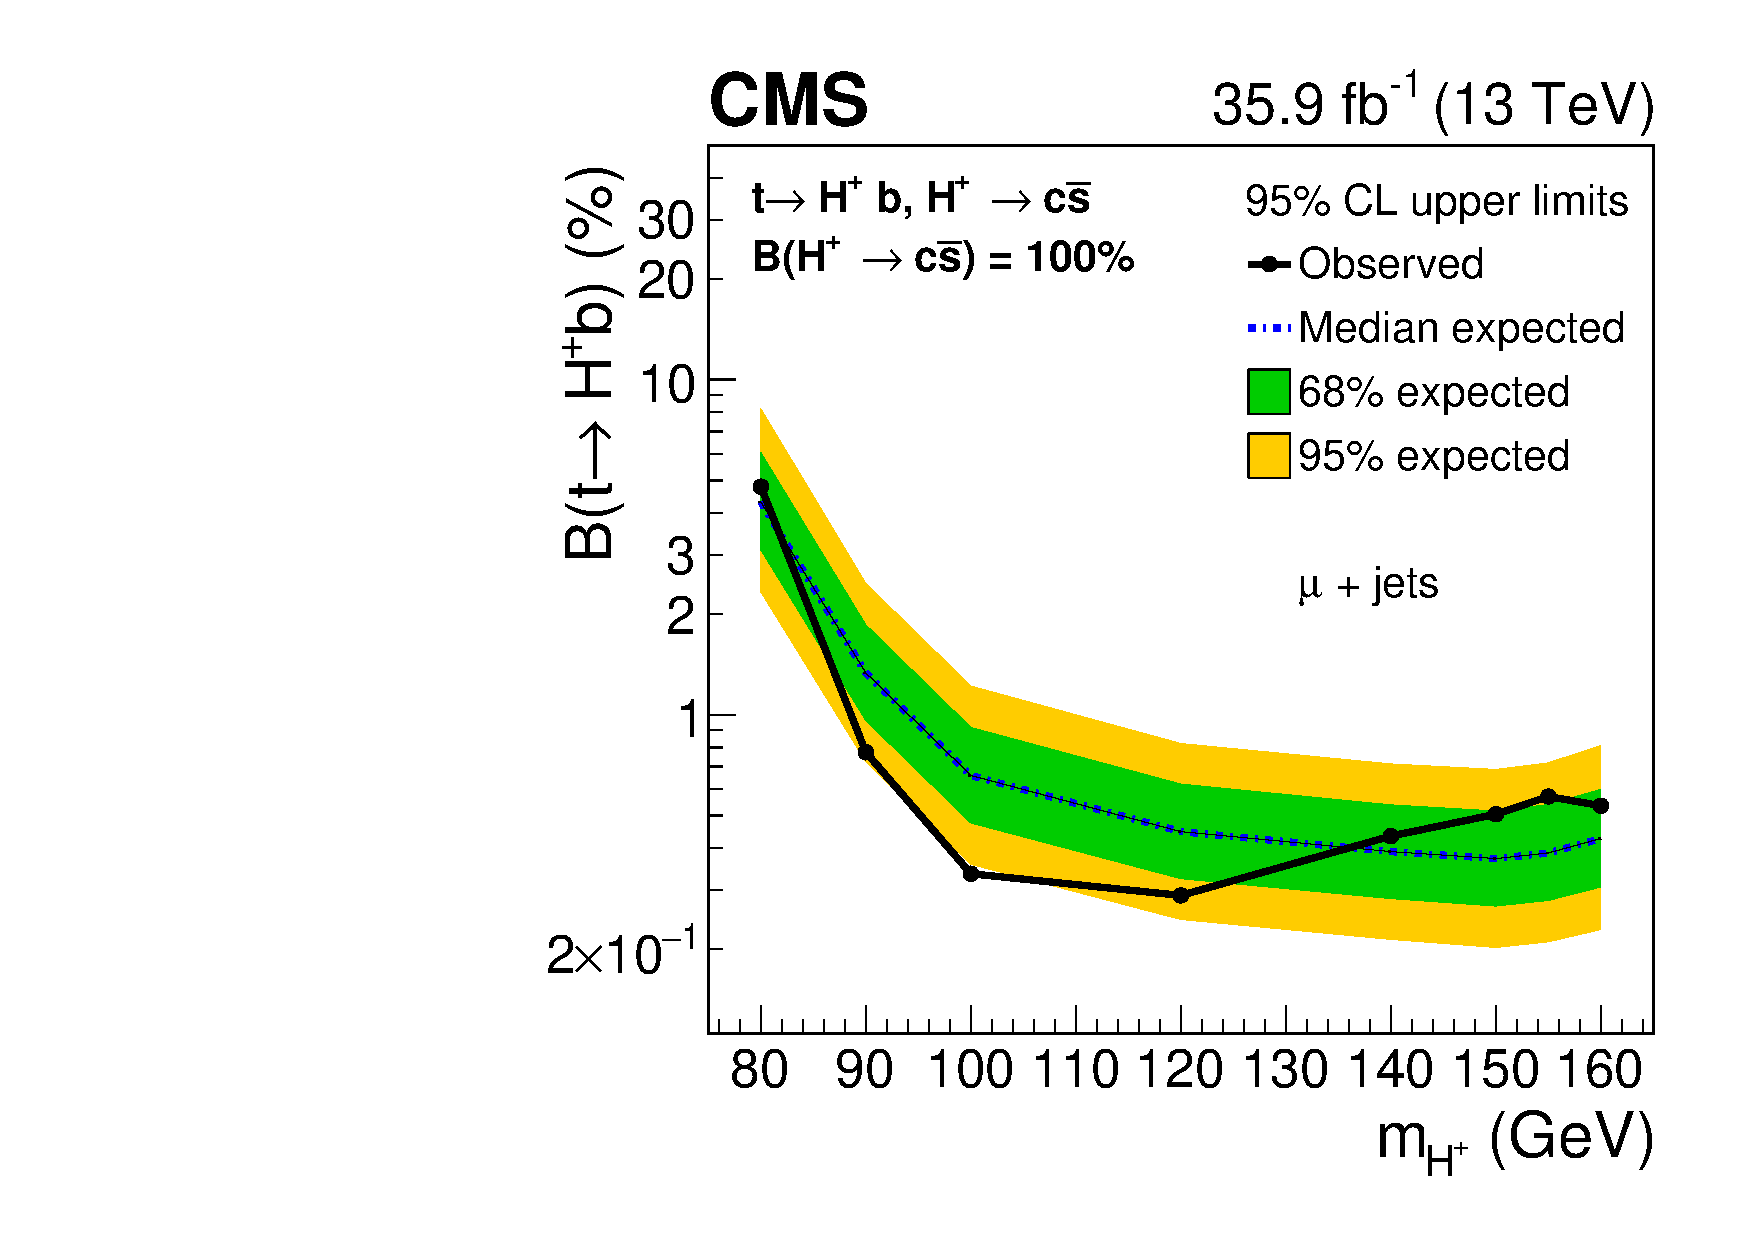
\includegraphics[width=0.30\linewidth]{Image/Limit/limit_pdf/limit_mu_Cat2_cTagInc.pdf}}
    \subfigure[With loose \PQc tagging \label{subfig:limit_ele_cTagL}]
    {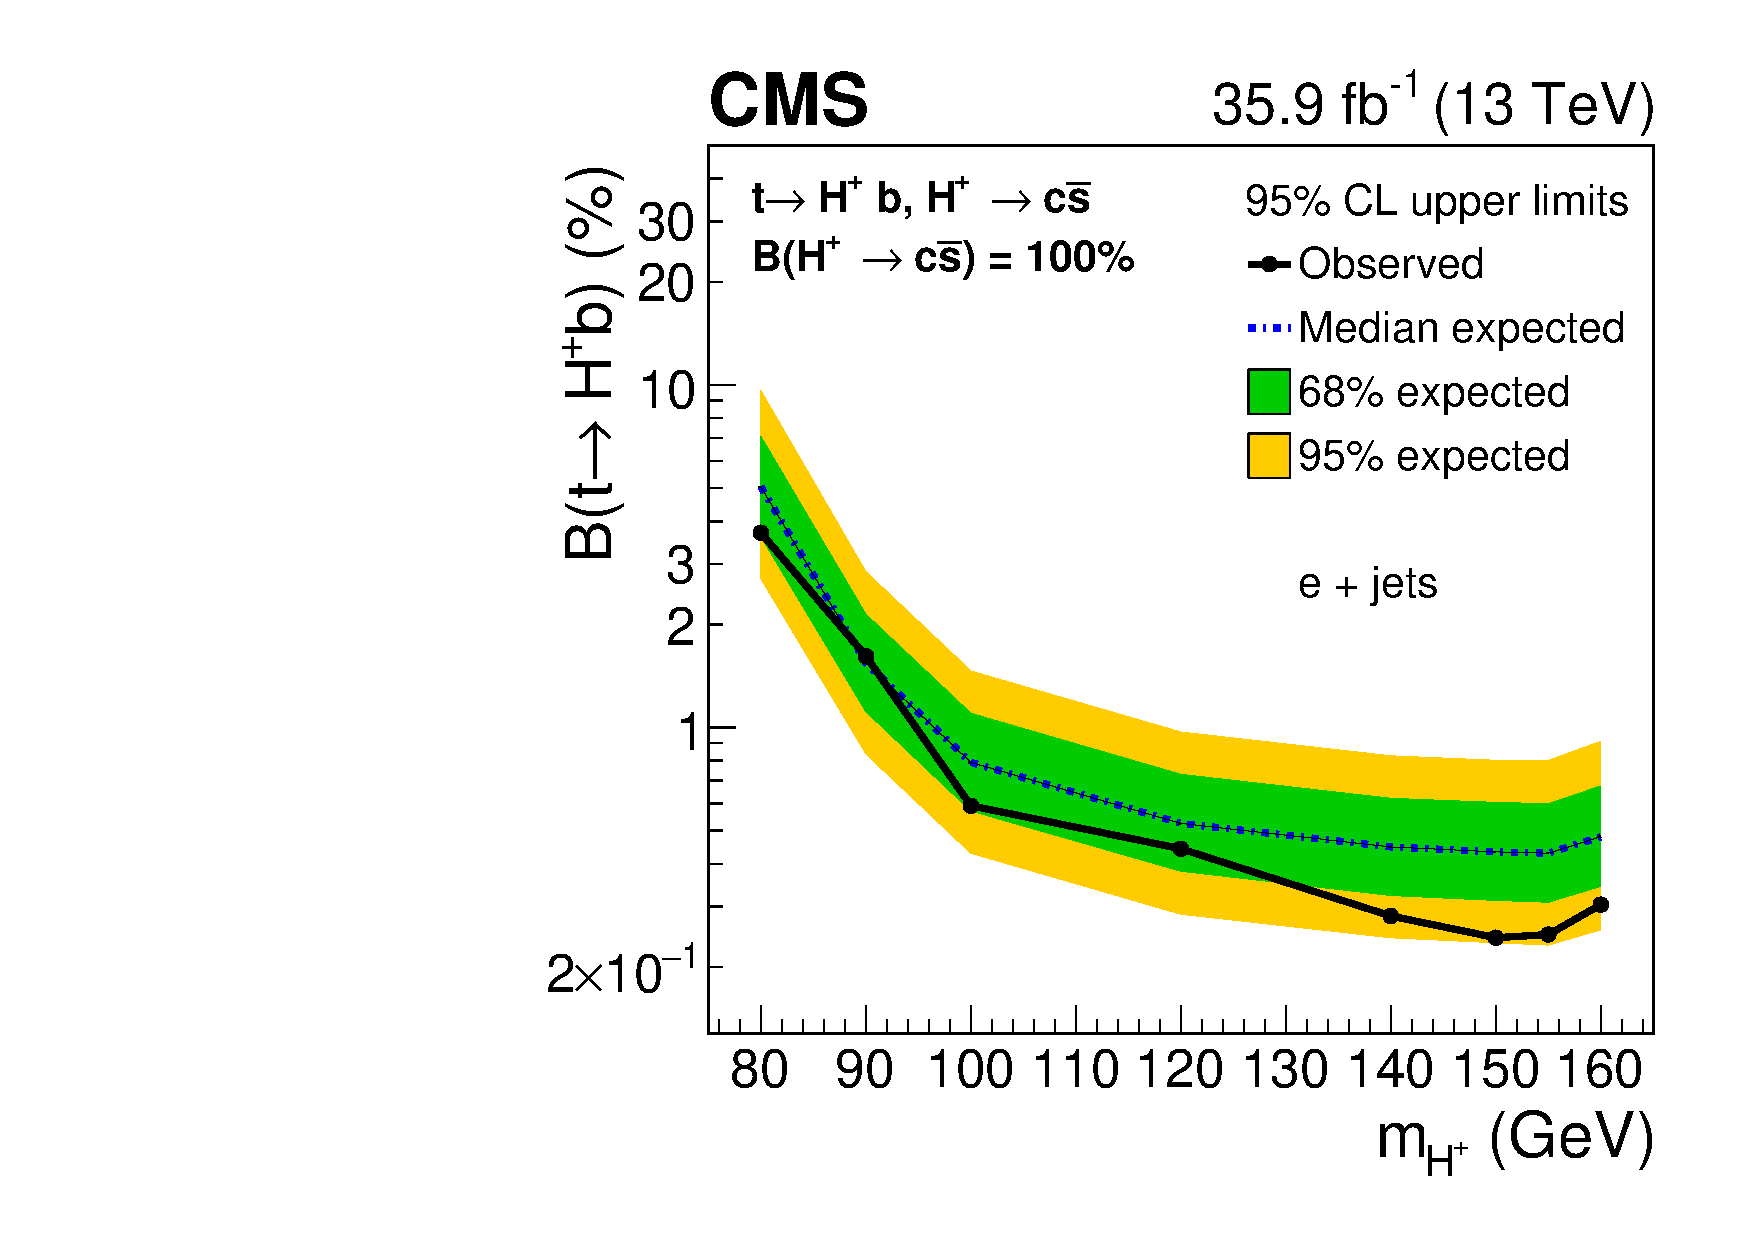
\includegraphics[width=0.30\linewidth]{Image/Limit/limit_pdf/limit_ele_Cat2_cTagInc.pdf}}
    \subfigure[With loose \PQc tagging \label{subfig:limit_lep_cTagL}]
    {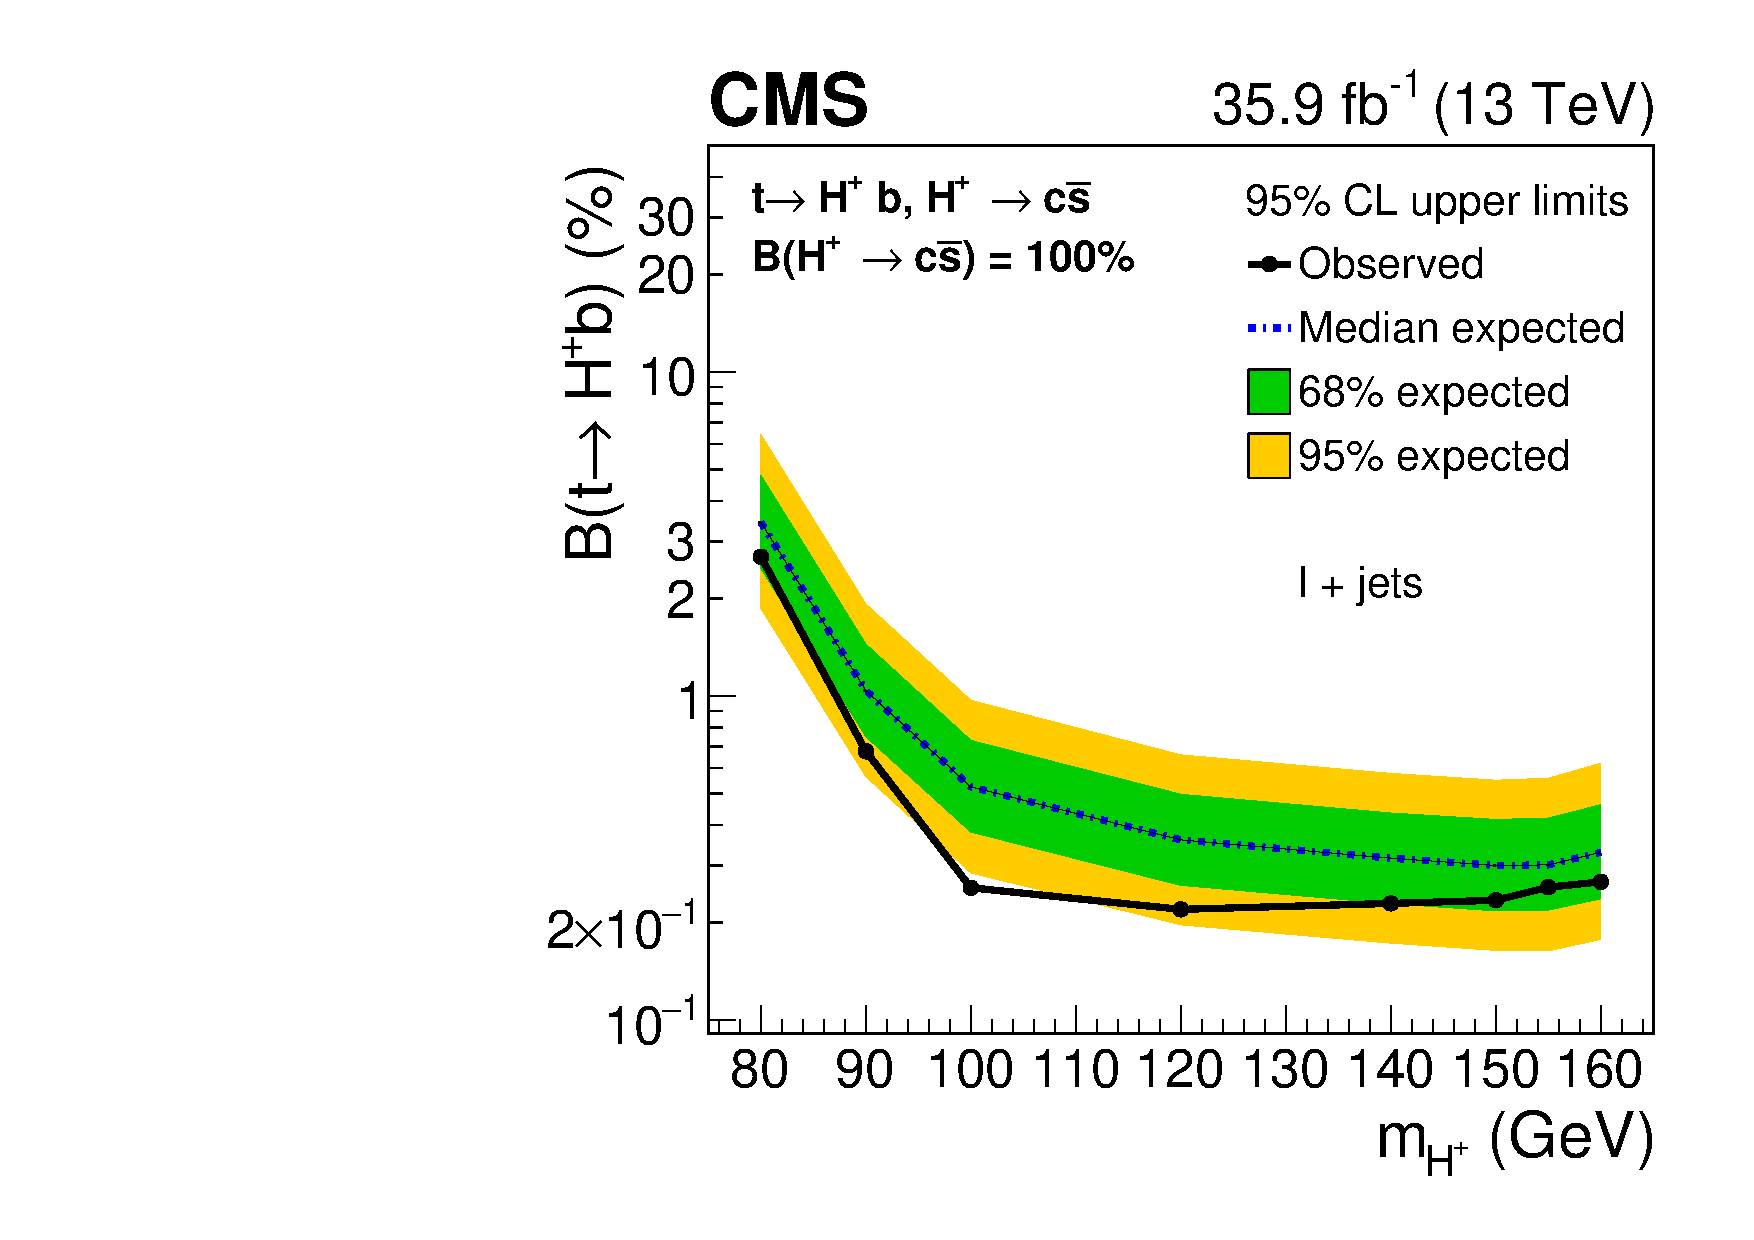
\includegraphics[width=0.30\linewidth]{Image/Limit/limit_pdf/limit_mu_ele_Cat2_cTagInc.pdf}}
\caption{The upper limit in \% on \brThb as a function of $m_{H^{+}}$ using $\mjj$ after kinematic fit
	selection without \PQc tagging, and with loose \PQc tagging, as discussed in 
	Section~\ref{ss:mjj_Inc} and \ref{ss:mjj_cTagL}, for \mujets, \ejets, and \ljets channel.}
    \label{fig:limit_cTagL}
\end{figure}


%-----------------------------------------
\subsection{Limits from inclusive event category with loose \text{c} tagging}
\label{ss:limit_cTagL}
%-----------------------------------------
The $\mjj$ distribution from the events with inclusive loose \PQc tagging as discussed 
in Section~\ref{ss:mjj_cTagL} are used to compute upper limits as shown in
Figures~\ref{subfig:limit_mu_cTagL}, \ref{subfig:limit_ele_cTagL}, and \ref{subfig:limit_lep_cTagL}. 
From these figures, it can be seen that the limits are marginally better compared to that 
of Figures~\ref{subfig:limit_mu_Inc}, ~\ref{subfig:limit_ele_Inc}, and \ref{subfig:limit_lep_Inc}. 
For different charged Higgs masses, the expected (observed) limits for loose \PQc tagging are in the 
range 0.37--4.32\% (0.29--4.79\%), 0.43--5.04\% (0.24--3.70\%), and 
0.30--3.44 (0.22--2.69\%)
for \mujets, \ejets, and \ljets channel, respectively.

%-----------------------------------------
\subsection{Limits from exclusive event categories based on \text{c} tagging}
\label{ss:limit_cTagEx}
%-----------------------------------------
\begin{figure}
    \centering  
    \subfigure[From combined exclusive charm categories.]
    {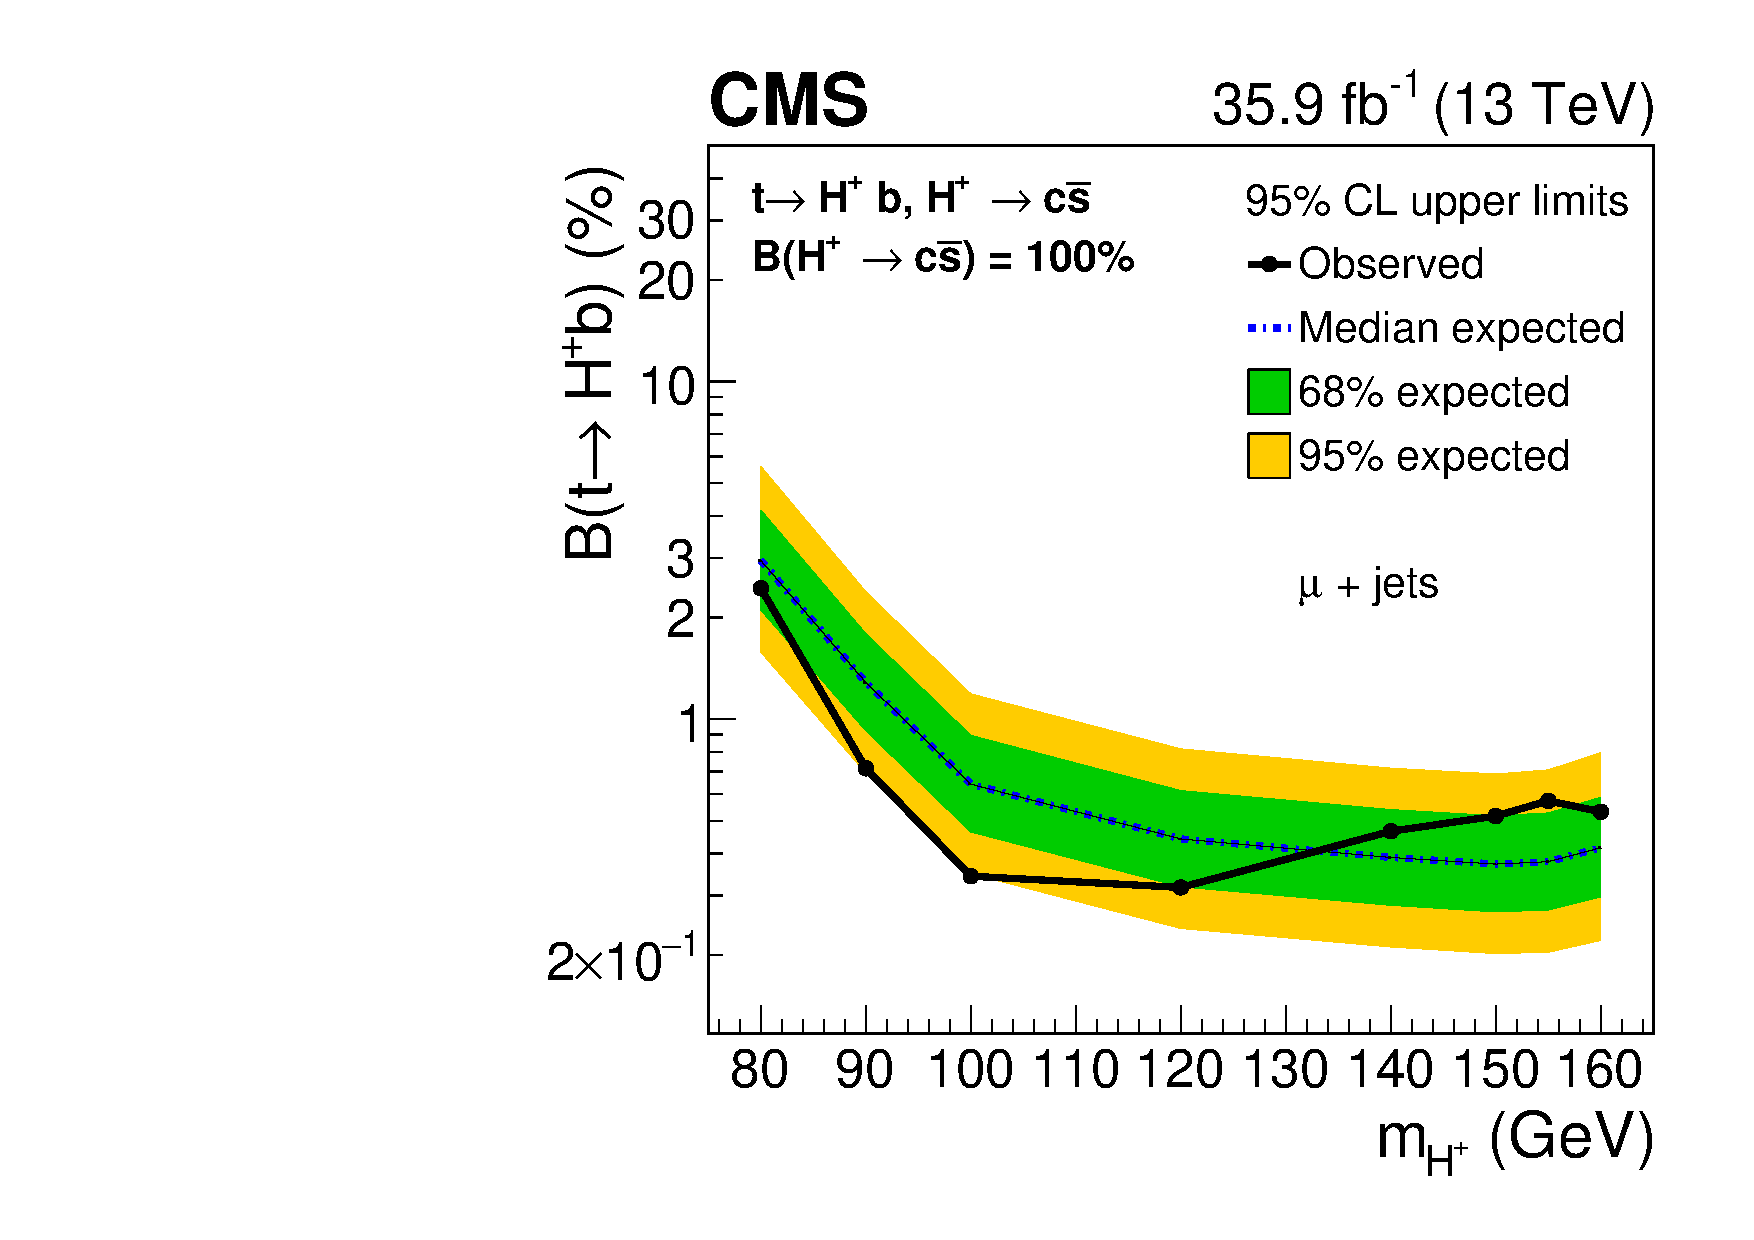
\includegraphics[width=0.45\linewidth]{Image/Limit/limit_pdf/limit_mu_Cat3_cTagEx.pdf}}
    \subfigure[From combined exclusive charm categories.]
    {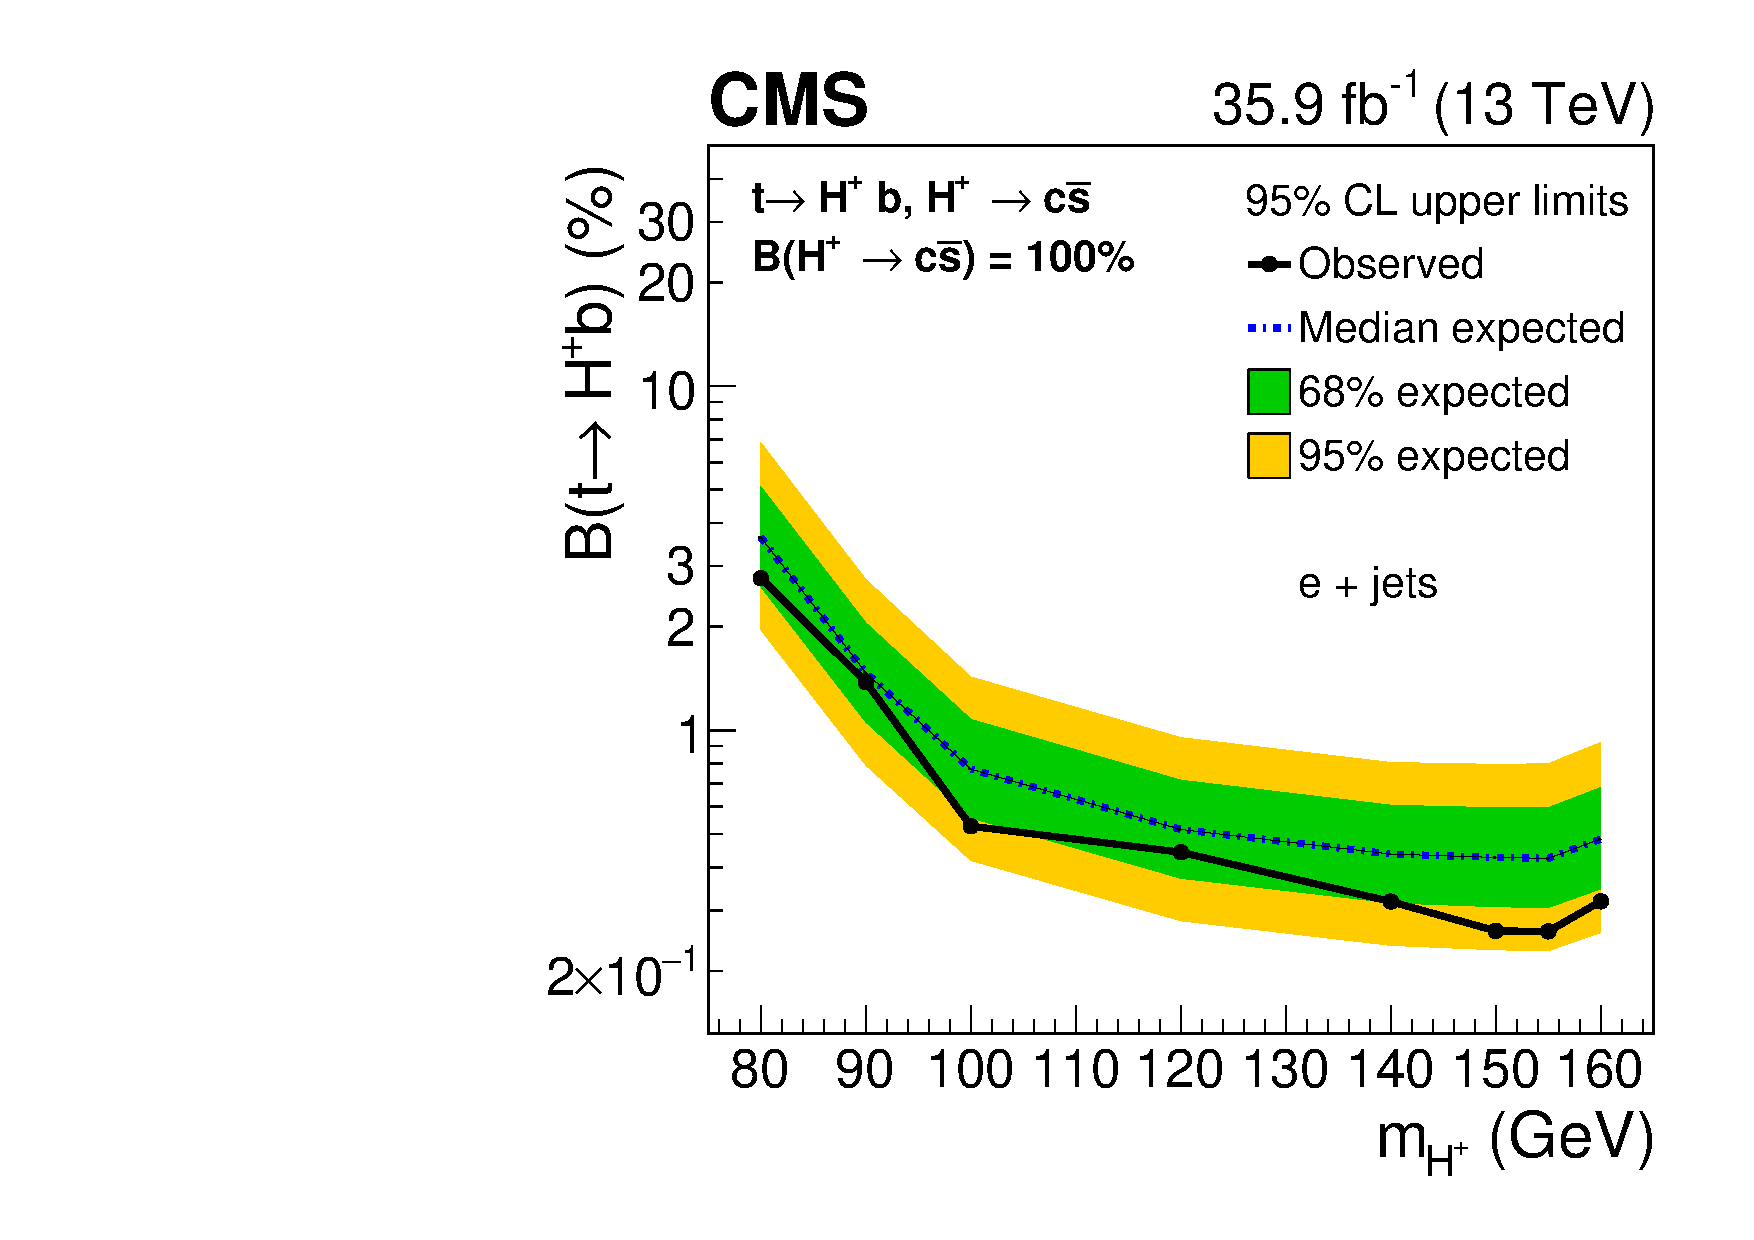
\includegraphics[width=0.45\linewidth]{Image/Limit/limit_pdf/limit_ele_Cat3_cTagEx.pdf}}
    \vfil
    \subfigure[From combined exclusive charm categories.]
    {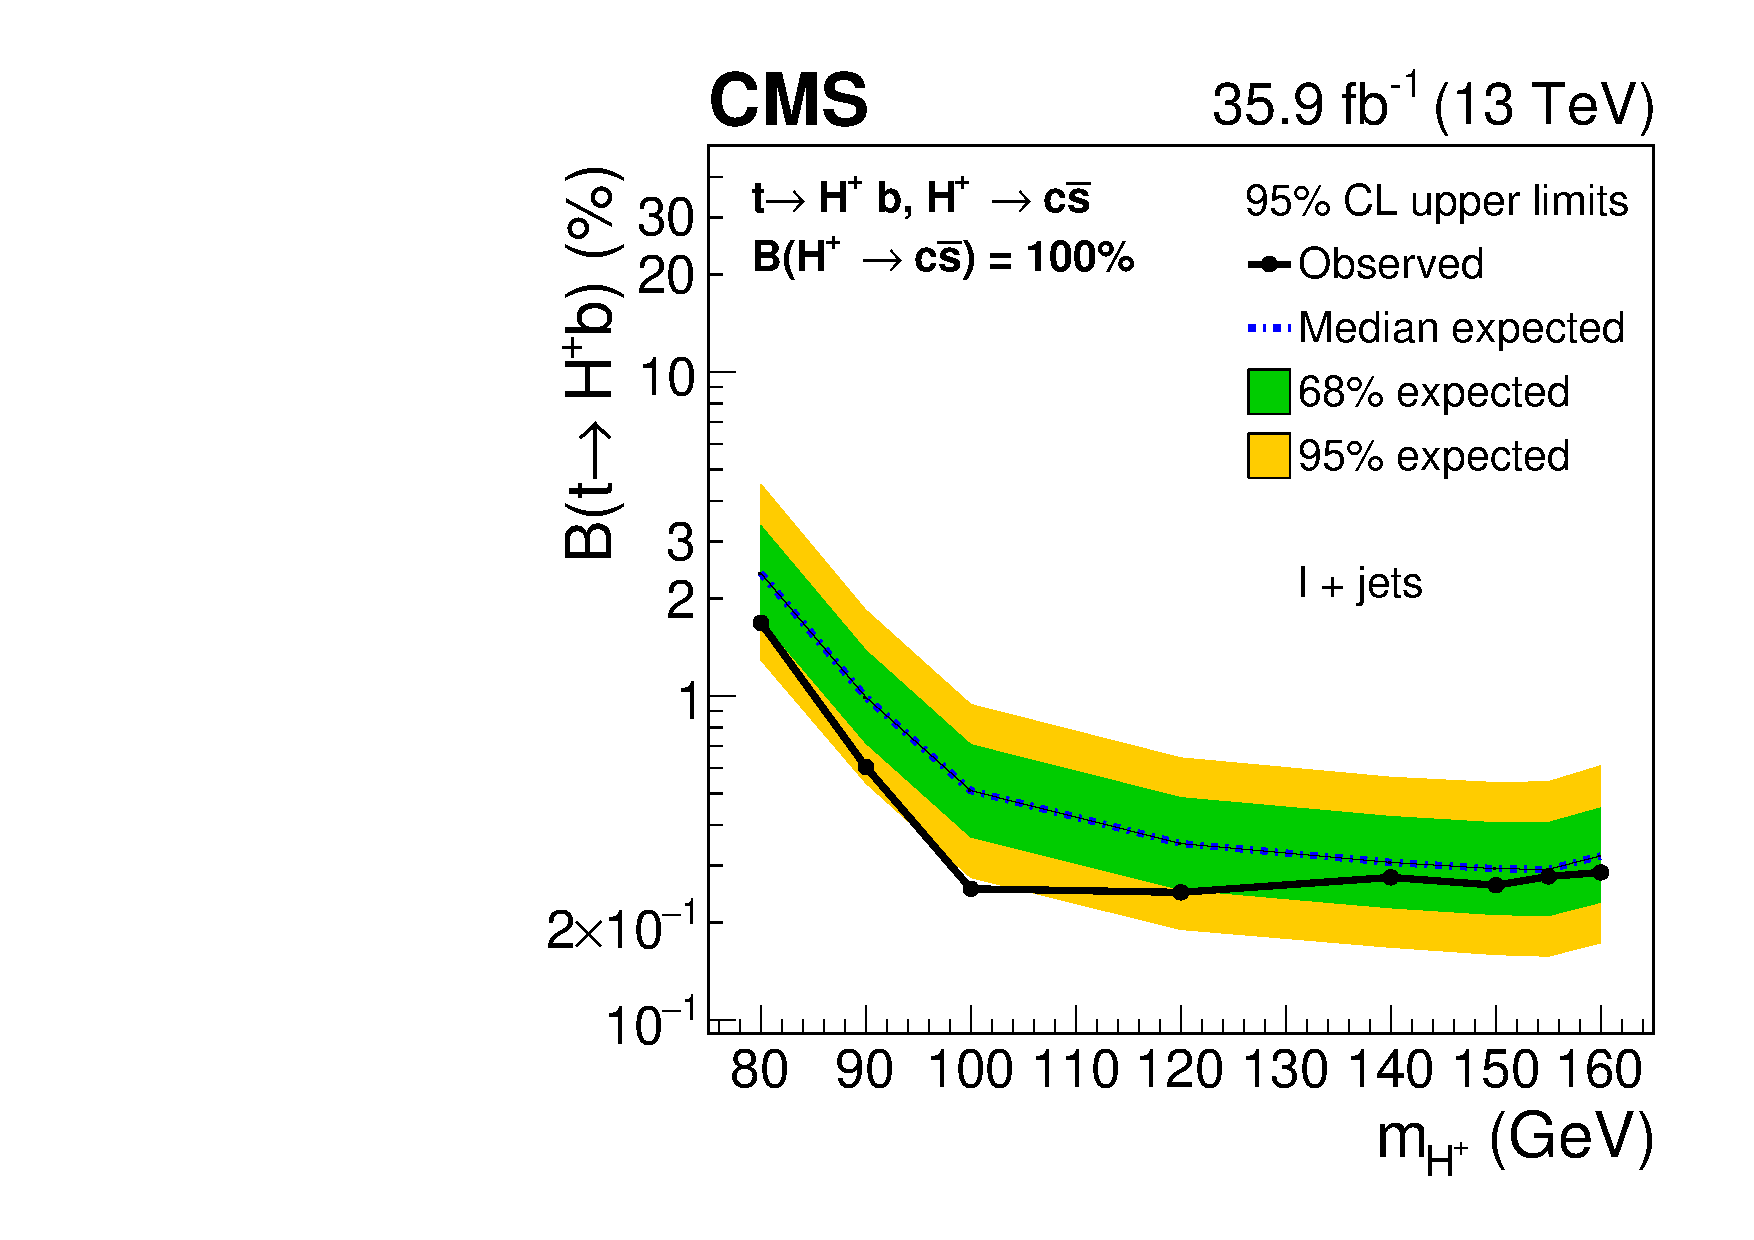
\includegraphics[width=0.60\linewidth]{Image/Limit/limit_pdf/limit_mu_ele_Cat3_cTagEx.pdf}}
	\caption{The upper limit in \% on \brThb as a function of $m_{H^{+}}$ by combining \mjj 
	distributions from different exclusive charm categories as discussed in 
	Section~\ref{ss:mjj_cTagEx} for \mujets \ejets, and \ljets channel.}
    \label{fig:limit_cTagEx}
\end{figure}

The signal significance is different in different charm categories as described in 
Section~\ref{ss:mjj_cTagEx}. The $\mjj$ distributions from loose, medium, and tight 
exclusive charm tagging categories are combined to compute the expected limits as shown in 
Figure~\ref{fig:limit_cTagEx}. From this figure, it can be seen that the upper limits
from exclusive categories are better compared to that obtained from inclusive working points.
For different charged Higgs masses, the expected (observed) limits from combined categories are 
in the range 0.37--2.95\% (0.32--2.44\%), 0.42--3.63\% (0.26--2.77\%), 
and 0.29--2.39\% (0.25--1.68) for \mujets, \ejets, and \ljets channel, 
respectively.

\begin{figure}
    \centering  
    \subfigure[Expected limits.]
    {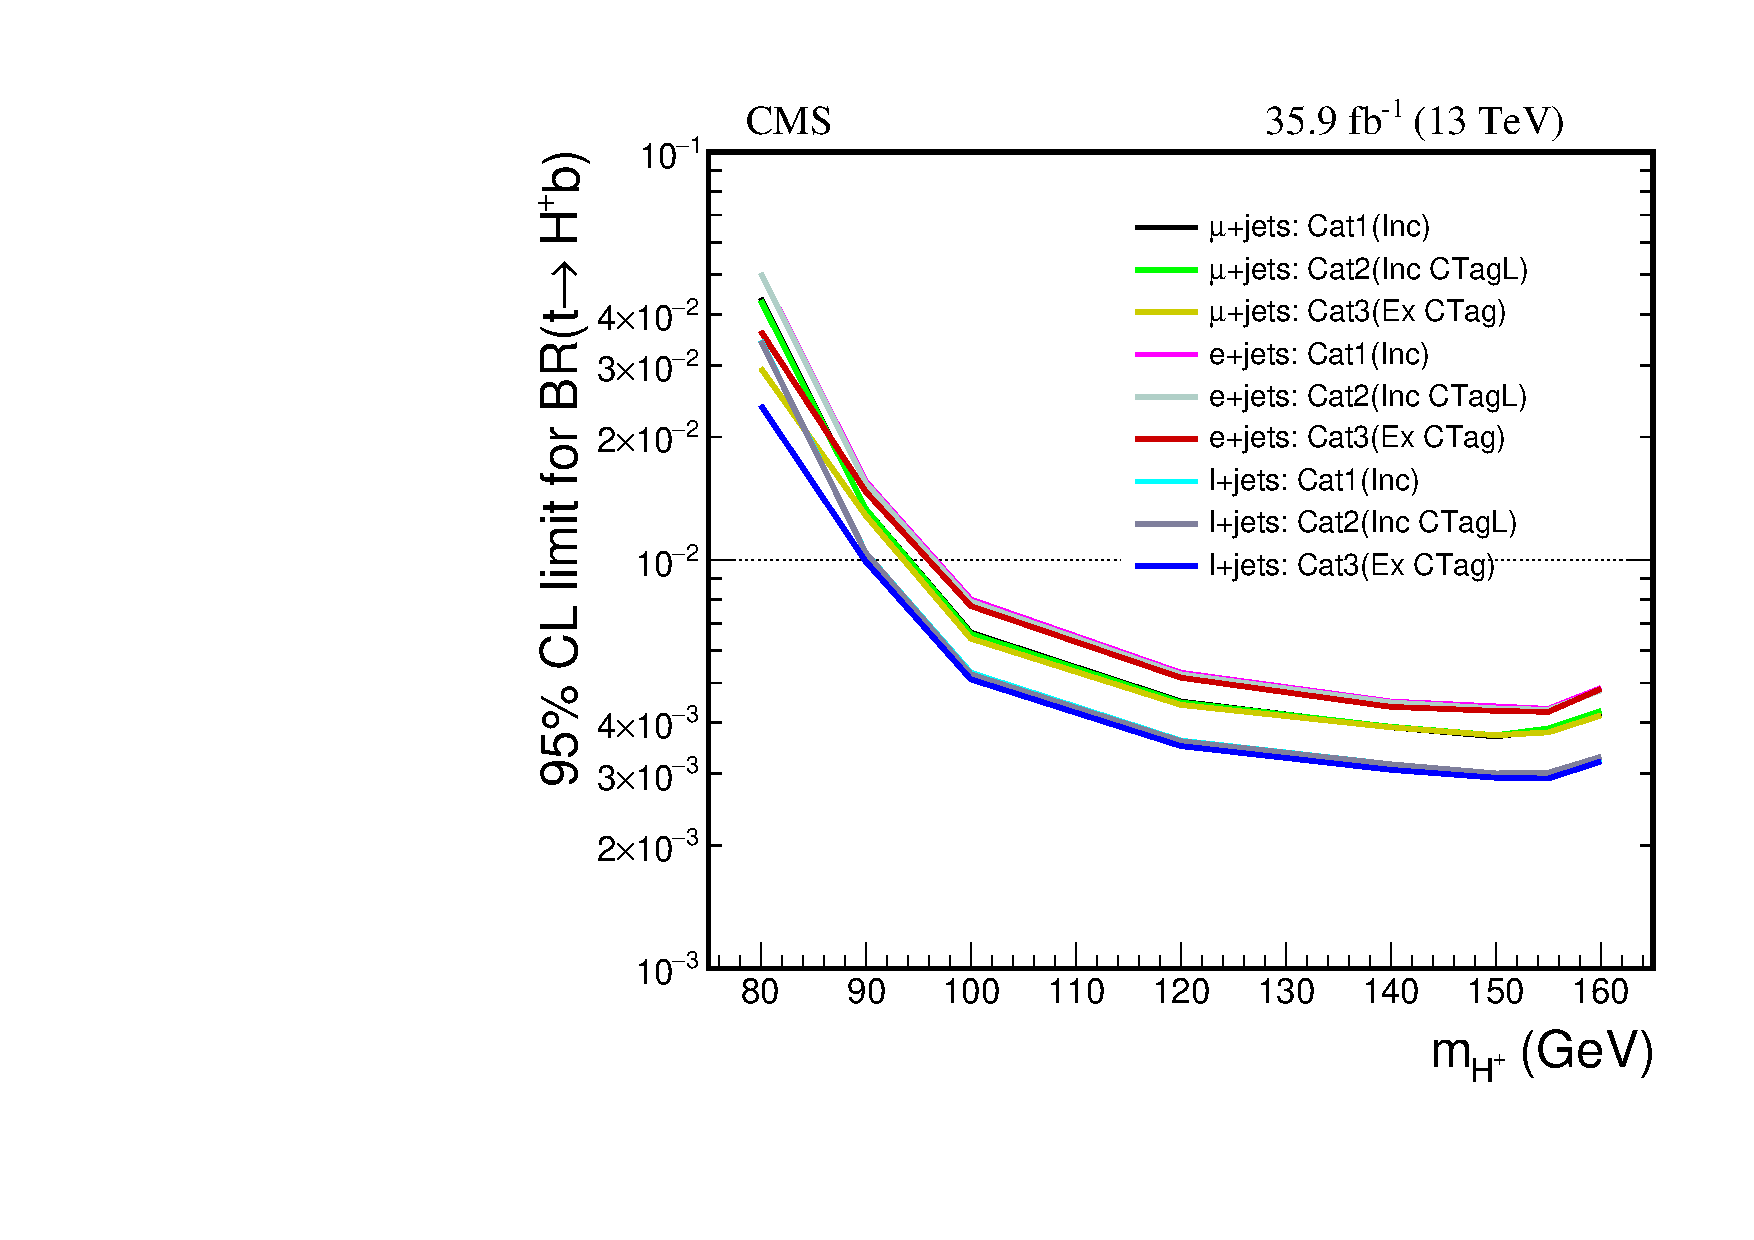
\includegraphics[width=0.6\linewidth]{Image/Limit/all_limits_expected.pdf}}
    \vfil
    \subfigure[Observed limits.]
    {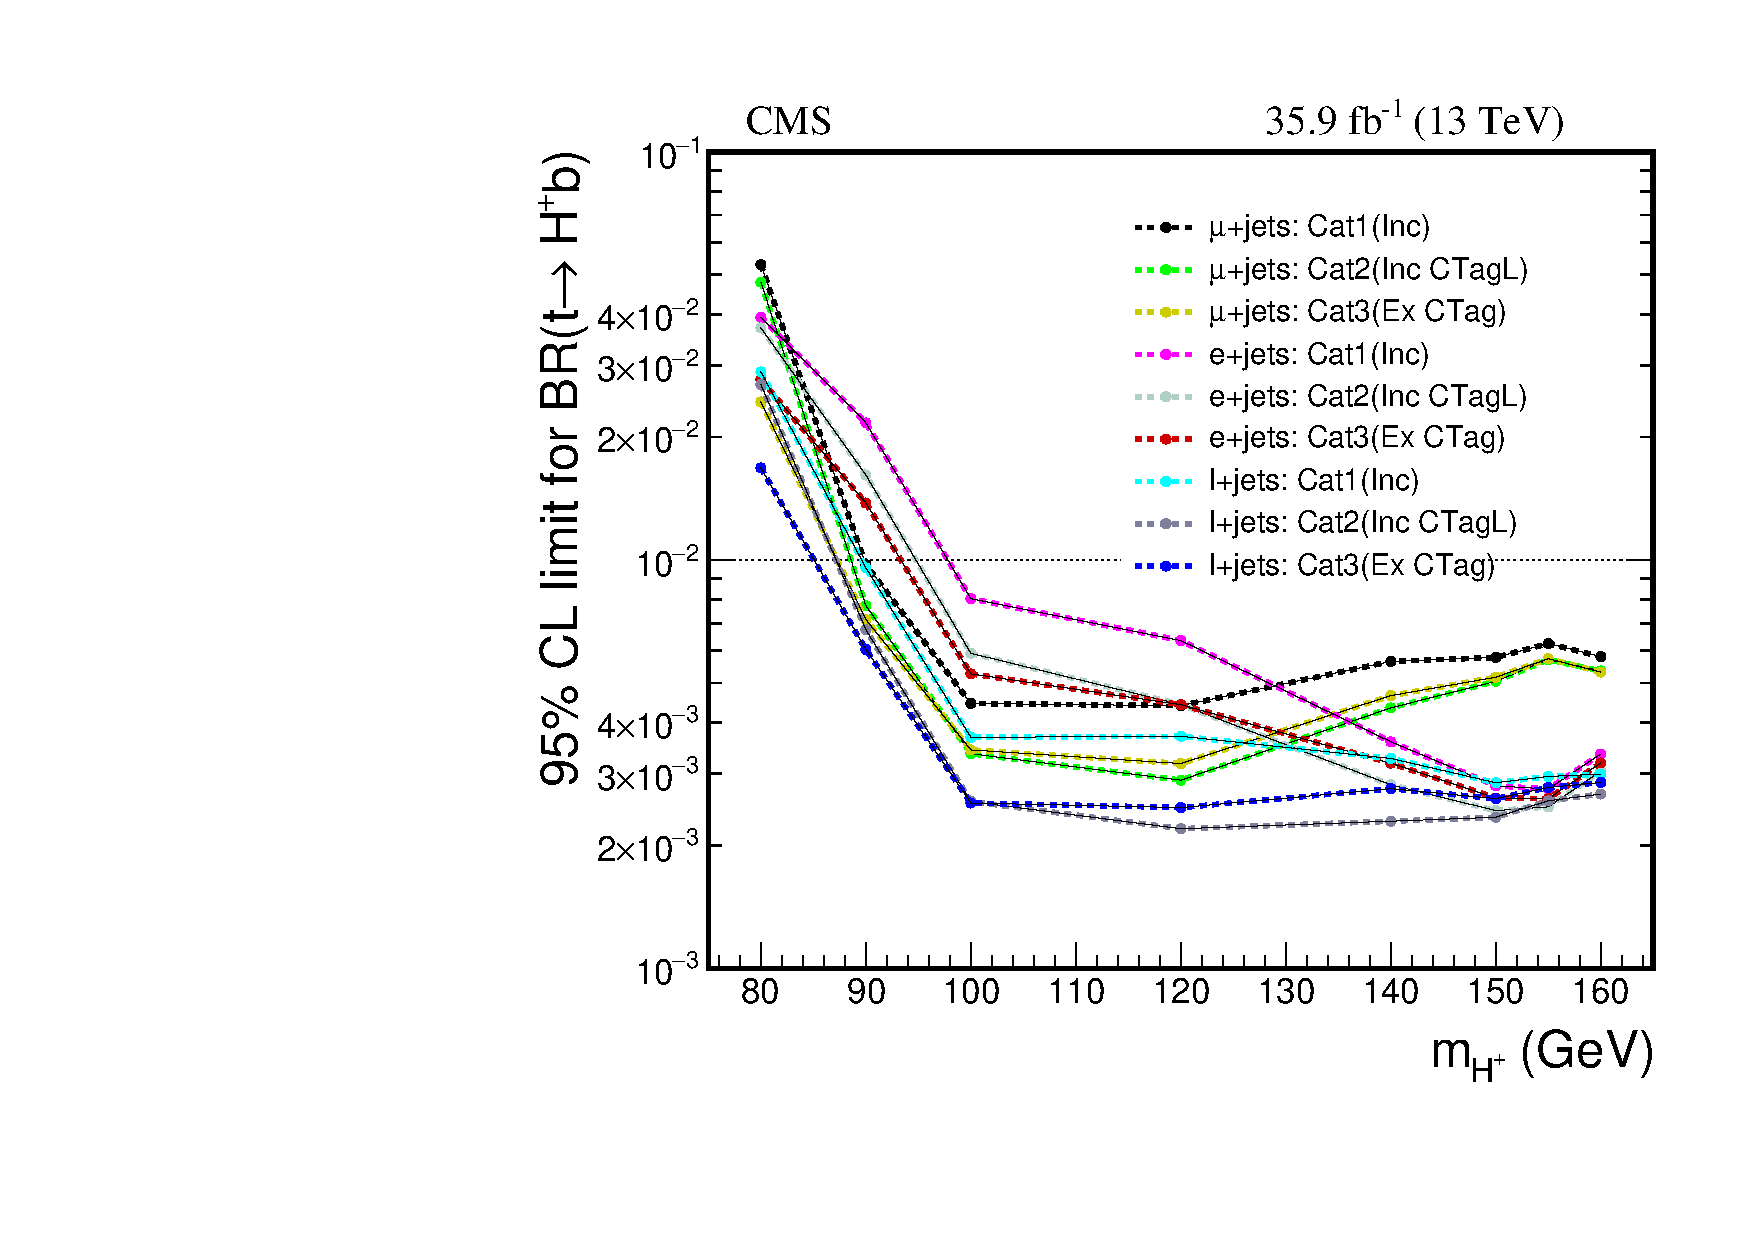
\includegraphics[width=0.6\linewidth]{Image/Limit/all_limits_observed.pdf}}
    \caption{The upper limit in \% on \brThb as a function of $m_{H^{+}}$ using $\mjj$ from 
	all event categories for \mujets, \ejets, and \ljets channel.}
\label{fig:finalLimit}
\end{figure}

\begin{table}
\caption{95\% CL exclusion limit in \% for \mujets channel from different event categories.}
\label{tab:limitMu}
\begin{center}
\begin{tabular}{ ccccccc}
\hline 
\hline 
\multicolumn{1}{c}{} & \multicolumn{2}{c}{$\mjj(Inc)$} & \multicolumn{2}{c}{$\mjj(Inc ~CTagL)$} & \multicolumn{2}{c}{$\mjj(Ex ~CTag)$} \\
  
{\bf{$m_{H^+}$}} & Expected & Observed & Expected & Observed & Expected & Observed  \\ 
  
  (\GeV) & (\%) & (\%) & (\%) & (\%) & (\%) & (\%)  \\ 
 \hline 
\hline 
80  & $4.38^{+1.76}_{-1.23}$&5.29
 & $4.32^{+1.74}_{-1.21}$&4.79
 & $2.95^{+1.21}_{-0.85}$&2.44
\\
  
90  & $1.33^{+0.52}_{-0.37}$&0.97
 & $1.33^{+0.52}_{-0.37}$&0.77
 & $1.28^{+0.51}_{-0.36}$&0.72
\\
  
100  & $0.66^{+0.26}_{-0.18}$&0.45
 & $0.66^{+0.26}_{-0.18}$&0.34
 & $0.64^{+0.25}_{-0.18}$&0.34
\\
  
120  & $0.45^{+0.17}_{-0.13}$&0.44
 & $0.45^{+0.17}_{-0.12}$&0.29
 & $0.44^{+0.17}_{-0.12}$&0.32
\\
  
140  & $0.39^{+0.15}_{-0.11}$&0.56
 & $0.39^{+0.15}_{-0.11}$&0.43
 & $0.39^{+0.15}_{-0.11}$&0.47
\\
  
150  & $0.37^{+0.14}_{-0.10}$&0.58
 & $0.37^{+0.14}_{-0.10}$&0.50
 & $0.37^{+0.15}_{-0.10}$&0.52
\\
  
155  & $0.38^{+0.15}_{-0.11}$&0.62
 & $0.39^{+0.15}_{-0.11}$&0.57
 & $0.38^{+0.15}_{-0.11}$&0.57
\\
  
160  & $0.42^{+0.17}_{-0.12}$&0.58
 & $0.43^{+0.17}_{-0.12}$&0.54
 & $0.42^{+0.17}_{-0.12}$&0.53
\\
\hline 
\end{tabular}
\end{center}
\end{table}

\begin{table}
\caption{95\% CL exclusion limit in \% for \ejets channel from different event categories.}
\label{tab:limitEle}
\begin{center}
\begin{tabular}{ ccccccc}
\hline 
\hline 
\multicolumn{1}{c}{} & \multicolumn{2}{c}{$\mjj(Inc)$} & \multicolumn{2}{c}{$\mjj(Inc ~CTagL)$} & \multicolumn{2}{c}{$\mjj(Ex ~CTag)$} \\
  
{\bf{$m_{H^+}$}} & Expected & Observed & Expected & Observed & Expected & Observed  \\ 
  
  (\GeV) & (\%) & (\%) & (\%) & (\%) & (\%) & (\%)  \\ 
 \hline 
\hline 
80  & $5.04^{+2.05}_{-1.42}$&3.94
 & $5.04^{+2.03}_{-1.43}$&3.70
 & $3.63^{+1.46}_{-1.02}$&2.77
\\
  
90  & $1.56^{+0.61}_{-0.43}$&2.17
 & $1.54^{+0.60}_{-0.43}$&1.62
 & $1.47^{+0.58}_{-0.41}$&1.38
\\
  
100  & $0.80^{+0.31}_{-0.22}$&0.80
 & $0.79^{+0.31}_{-0.22}$&0.59
 & $0.77^{+0.30}_{-0.21}$&0.53
\\
  
120  & $0.53^{+0.20}_{-0.15}$&0.64
 & $0.52^{+0.21}_{-0.14}$&0.44
 & $0.52^{+0.20}_{-0.14}$&0.44
\\
  
140  & $0.45^{+0.17}_{-0.13}$&0.36
 & $0.45^{+0.17}_{-0.12}$&0.28
 & $0.44^{+0.17}_{-0.12}$&0.32
\\
  
150  & $0.44^{+0.17}_{-0.12}$&0.28
 & $0.43^{+0.17}_{-0.12}$&0.24
 & $0.43^{+0.17}_{-0.12}$&0.26
\\
  
155  & $0.43^{+0.17}_{-0.12}$&0.27
 & $0.43^{+0.17}_{-0.12}$&0.25
 & $0.42^{+0.17}_{-0.12}$&0.26
\\
  
160  & $0.49^{+0.20}_{-0.14}$&0.33
 & $0.48^{+0.20}_{-0.14}$&0.30
 & $0.48^{+0.20}_{-0.14}$&0.32
\\
\hline 
\end{tabular}
\end{center}
\end{table}

\begin{table}
\caption{95\% CL exclusion limit in \% for \ljets channel from different event categories.}
\label{tab:limitLep}
\begin{center}
\begin{tabular}{ ccccccc}
\hline 
\hline 
\multicolumn{1}{c}{} & \multicolumn{2}{c}{$\mjj(Inc)$} & \multicolumn{2}{c}{$\mjj(Inc ~CTagL)$} & \multicolumn{2}{c}{$\mjj(Ex ~CTag)$} \\
  
{\bf{$m_{H^+}$}} & Expected & Observed & Expected & Observed & Expected & Observed  \\ 
  
  (\GeV) & (\%) & (\%) & (\%) & (\%) & (\%) & (\%)  \\ 
 \hline 
\hline 
80  & $3.45^{+1.36}_{-0.97}$&2.89
 & $3.44^{+1.36}_{-0.96}$&2.69
 & $2.39^{+0.96}_{-0.67}$&1.68
\\
  
90  & $1.04^{+0.41}_{-0.29}$&0.96
 & $1.04^{+0.41}_{-0.29}$&0.68
 & $0.99^{+0.39}_{-0.28}$&0.60
\\
  
100  & $0.53^{+0.20}_{-0.15}$&0.37
 & $0.52^{+0.21}_{-0.14}$&0.26
 & $0.51^{+0.20}_{-0.14}$&0.25
\\
  
120  & $0.36^{+0.14}_{-0.10}$&0.37
 & $0.36^{+0.14}_{-0.10}$&0.22
 & $0.35^{+0.14}_{-0.10}$&0.25
\\
  
140  & $0.32^{+0.12}_{-0.09}$&0.33
 & $0.32^{+0.12}_{-0.09}$&0.23
 & $0.31^{+0.12}_{-0.08}$&0.28
\\
  
150  & $0.30^{+0.11}_{-0.08}$&0.28
 & $0.30^{+0.12}_{-0.08}$&0.23
 & $0.29^{+0.11}_{-0.08}$&0.26
\\
  
155  & $0.30^{+0.12}_{-0.08}$&0.30
 & $0.30^{+0.12}_{-0.08}$&0.26
 & $0.29^{+0.12}_{-0.08}$&0.28
\\
  
160  & $0.33^{+0.13}_{-0.09}$&0.30
 & $0.33^{+0.13}_{-0.09}$&0.27
 & $0.32^{+0.13}_{-0.09}$&0.29
\\
\hline 
\end{tabular}
\end{center}
\end{table}

